\documentclass{article}

\usepackage{tikz}

\begin{document}

  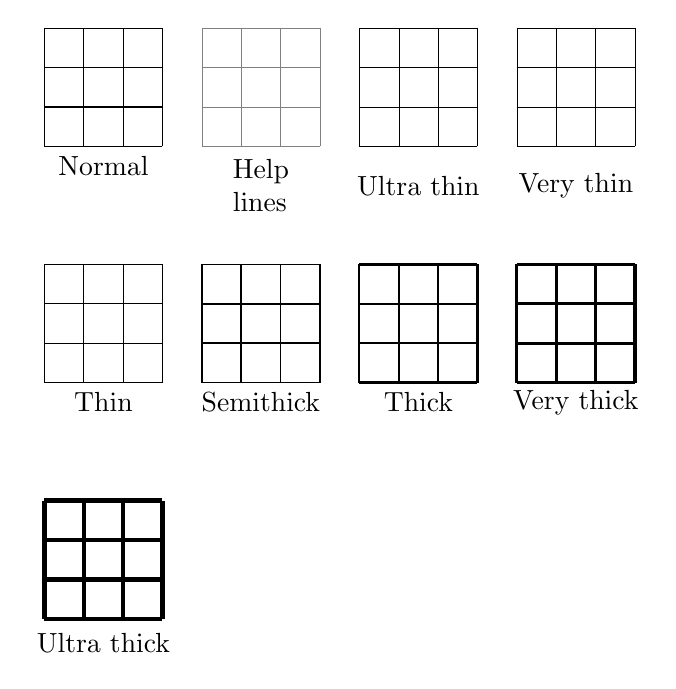
\begin{tikzpicture}

    \draw[step=0.5] (0,0) grid (1.5,1.5);

    \node at (0.75,-0.25) {Normal};



    \begin{scope}[xshift=2cm]

      \draw[help lines,step=0.5] (0,0) grid (1.5,1.5);

      \node[align=left] at (0.75,-0.5)
      {Help \\
        lines};

    \end{scope}



    \begin{scope}[xshift=4cm]

      \draw[ultra thin,step=0.5] (0,0) grid (1.5,1.5);

      \node at (0.75,-0.5) {Ultra thin};

    \end{scope}



    \begin{scope}[xshift=6cm]

      \draw[very thin,step=0.5] (0,0) grid (1.5,1.5);

      \node at (0.75,-0.5) {Very thin};

    \end{scope}





    \begin{scope}[yshift=-3cm]

      \draw[thin,step=0.5] (0,0) grid (1.5,1.5);

      \node at (0.75,-0.25) {Thin};

    \end{scope}



    \begin{scope}[xshift=2cm,yshift=-3cm]

      \draw[semithick,step=0.5] (0,0) grid (1.5,1.5);

      \node at (0.75,-0.25) {Semithick};

    \end{scope}



    \begin{scope}[xshift=4cm,yshift=-3cm]

      \draw[thick,step=0.5] (0,0) grid (1.5,1.5);

      \node at (0.75,-0.25) {Thick};

    \end{scope}



    \begin{scope}[xshift=6cm,yshift=-3cm]

      \draw[very thick,step=0.5] (0,0) grid (1.5,1.5);

      \node at (0.75,-0.25) {Very thick};

    \end{scope}





    \begin{scope}[yshift=-6cm]

      \draw[ultra thick,step=0.5] (0,0) grid (1.5,1.5);

      \node at (0.75,-0.3) {Ultra thick};

    \end{scope}

  \end{tikzpicture}

\end{document}